%%%%%%%%%%%%%%%%%%%%%%%%%%%%%%%%%%%%%%%%%
% Classicthesis Typographic Thesis
% LaTeX Template
% Version 1.4 (1/1/16)
%
% This template has been downloaded from:
% http://www.LaTeXTemplates.com
%
% Original author:
% André Miede (http://www.miede.de) with commenting modifications by:
% Vel (vel@LaTeXTemplates.com)
%
% License:
% GNU General Public License (v2)
%
% General Tips:
% 1) Make sure to edit the classicthesis-config.file
% 2) New enumeration (A., B., C., etc in small caps): \begin{aenumerate} \end{aenumerate}
% 3) For margin notes: \marginpar or \graffito{}
% 4) Do not use bold fonts in this style, it is designed around them
% 5) Use tables as in the examples
% 6) See classicthesis-preamble.sty for useful commands
%
%%%%%%%%%%%%%%%%%%%%%%%%%%%%%%%%%%%%%%%%%

%----------------------------------------------------------------------------------------
%	PACKAGES AND OTHER DOCUMENT CONFIGURATIONS
%----------------------------------------------------------------------------------------

\documentclass[
		twoside,openright,titlepage,numbers=noenddot,headinclude,%1headlines,
	 	footinclude=true,cleardoublepage=empty,
		dottedtoc, % Make page numbers in the table of contents flushed right with dots leading to them
		BCOR=5mm,paper=a4,fontsize=11pt, % Binding correction, paper type and font size
		ngerman,american, % Languages, change this to your language(s)
		]{scrreprt}

% Includes the file which contains all the document configurations and packages - make sure to edit this file
%%%%%%%%%%%%%%%%%%%%%%%%%%%%%%%%%%%%%%%%%
% Classicthesis Typographic Thesis
% Configuration File
%
% This file has been downloaded from:
% http://www.LaTeXTemplates.com
%
% Original author:
% André Miede (http://www.miede.de) with extensive commenting changes by:
% Vel (vel@LaTeXTemplates.com)
%
% License:
% GNU General Public License (v2)
%
% Important note:
% The main lines to change in this file are in the DOCUMENT VARIABLES
% section, the rest of the file is for advanced configuration.
%
%%%%%%%%%%%%%%%%%%%%%%%%%%%%%%%%%%%%%%%%%

%----------------------------------------------------------------------------------------
%	CHARACTER ENCODING
%----------------------------------------------------------------------------------------

%\PassOptionsToPackage{utf8}{inputenc} % Set the encoding of your files. UTF-8 is the only sensible encoding nowadays. If you can't read äöüßáéçèê∂åëæƒÏ€ then change the encoding setting in your editor, not the line below. If your editor does not support utf8 use another editor!
\usepackage{inputenc}

%----------------------------------------------------------------------------------------
%	DOCUMENT VARIABLES
%	Fill in the lines below to enter your information into the thesis template
%	Each of the commands can be cited anywhere in the thesis
%----------------------------------------------------------------------------------------

% Remove drafting to get rid of the '[ Date - classicthesis version 4.0 ]' text at the bottom of every page
\PassOptionsToPackage{eulerchapternumbers,listings,drafting, pdfspacing, subfig,beramono,eulermath,parts}{classicthesis}
% Available options: drafting parts nochapters linedheaders eulerchapternumbers beramono eulermath pdfspacing minionprospacing tocaligned dottedtoc manychapters listings floatperchapter subfig

\newcommand{\myTitle}{Notes on Machine Learning\xspace}
\newcommand{\mySubtitle}{An Homage to The Elements of Typographic Style\xspace}
\newcommand{\myDegree}{Doktor-Ingenieur (Dr.-Ing.)\xspace}
\newcommand{\myName}{Herman Koe\xspace}
\newcommand{\myProf}{Put name here\xspace}
\newcommand{\myOtherProf}{Put name here\xspace}
\newcommand{\mySupervisor}{Put name here\xspace}
\newcommand{\myFaculty}{Put data here\xspace}
\newcommand{\myDepartment}{Put data here\xspace}
\newcommand{\myUni}{Put data here\xspace}
\newcommand{\myLocation}{Saarbrücken\xspace}
\newcommand{\myTime}{\today \xspace}
\newcommand{\myVersion}{version 4.2\xspace}

%----------------------------------------------------------------------------------------
%	USEFUL COMMANDS
%----------------------------------------------------------------------------------------

\newcommand{\ie}{i.\,e.}
\newcommand{\Ie}{I.\,e.}
\newcommand{\eg}{e.\,g.}
\newcommand{\Eg}{E.\,g.}

\newcounter{dummy} % Necessary for correct hyperlinks (to index, bib, etc.)
\providecommand{\mLyX}{L\kern-.1667em\lower.25em\hbox{Y}\kern-.125emX\@}
\newlength{\abcd} % for ab..z string length calculation

%----------------------------------------------------------------------------------------
%	PACKAGES
%----------------------------------------------------------------------------------------

\usepackage{lipsum} % Used for inserting dummy 'Lorem ipsum' text into the template

%------------------------------------------------

\PassOptionsToPackage{ngerman,american}{babel}  % Change this to your language(s)
% Spanish languages need extra options in order to work with this template
%\PassOptionsToPackage{spanish,es-lcroman}{babel}
%\usepackage{babel}

%------------------------------------------------			

\usepackage{csquotes}
\PassOptionsToPackage{%
%backend=biber, % Instead of bibtex
backend=bibtex8,bibencoding=ascii,%
language=auto,%
style=numeric-comp,%
%style=authoryear-comp, % Author 1999, 2010
%bibstyle=authoryear,dashed=false, % dashed: substitute rep. author with ---
sorting=nyt, % name, year, title
maxbibnames=10, % default: 3, et al.
%backref=true,%
natbib=true % natbib compatibility mode (\citep and \citet still work)
}{biblatex}
\usepackage{biblatex}

 %------------------------------------------------

\PassOptionsToPackage{fleqn}{amsmath} % Math environments and more by the AMS
 \usepackage{amsmath}

 %------------------------------------------------

\PassOptionsToPackage{T1}{fontenc} % T2A for cyrillics
\usepackage{fontenc}

%------------------------------------------------

\usepackage{textcomp} % Fix warning with missing font shapes

%------------------------------------------------

\usepackage{scrhack} % Fix warnings when using KOMA with listings package

%------------------------------------------------

\usepackage{xspace} % To get the spacing after macros right

%------------------------------------------------

\usepackage{mparhack} % To get marginpar right

%------------------------------------------------

\usepackage{fixltx2e} % Fixes some LaTeX stuff

%------------------------------------------------

\PassOptionsToPackage{smaller}{acronym} % Include printonlyused in the first bracket to only show acronyms used in the text
\usepackage{acronym} % Nice macros for handling all acronyms in the thesis

%\renewcommand*{\acsfont}[1]{\textssc{#1}} % For MinionPro
\renewcommand*{\aclabelfont}[1]{\acsfont{#1}}

%------------------------------------------------

\PassOptionsToPackage{pdftex}{graphicx}
\usepackage{graphicx}

%----------------------------------------------------------------------------------------
%	FLOATS: TABLES, FIGURES AND CAPTIONS SETUP
%----------------------------------------------------------------------------------------

\usepackage{tabularx} % Better tables
\setlength{\extrarowheight}{3pt} % Increase table row height
\newcommand{\tableheadline}[1]{\multicolumn{1}{c}{\spacedlowsmallcaps{#1}}}
\newcommand{\myfloatalign}{\centering} % To be used with each float for alignment
\usepackage{caption}
\captionsetup{font=small}
\usepackage{subfig}

%----------------------------------------------------------------------------------------
%	CODE LISTINGS SETUP
%----------------------------------------------------------------------------------------

\usepackage{listings}
%\lstset{emph={trueIndex,root},emphstyle=\color{BlueViolet}}%\underbar} % For special keywords
\lstset{language=[LaTeX]Tex,%C++ % Specify the language(s) for listings here
morekeywords={PassOptionsToPackage,selectlanguage},
keywordstyle=\color{RoyalBlue}, % Add \bfseries for bold
basicstyle=\small\ttfamily, % Makes listings a smaller font size and a different font
%identifierstyle=\color{NavyBlue}, % Color of text inside brackets
commentstyle=\color{Green}\ttfamily, % Color of comments
stringstyle=\rmfamily, % Font type to use for strings
numbers=left, % Change left to none to remove line numbers
numberstyle=\scriptsize, % Font size of the line numbers
stepnumber=5, % Increment of line numbers
numbersep=8pt, % Distance of line numbers from code listing
showstringspaces=false, % Sets whether spaces in strings should appear underlined
breaklines=true, % Force the code to stay in the confines of the listing box
%frameround=ftff, % Uncomment for rounded frame
%frame=single, % Frame border - none/leftline/topline/bottomline/lines/single/shadowbox/L
belowcaptionskip=.75\baselineskip % Space after the "Listing #: Desciption" text and the listing box
}

%----------------------------------------------------------------------------------------
%	HYPERREFERENCES
%----------------------------------------------------------------------------------------

\PassOptionsToPackage{pdftex,hyperfootnotes=false,pdfpagelabels}{hyperref}
\usepackage{hyperref}  % backref linktocpage pagebackref
\pdfcompresslevel=9
\pdfadjustspacing=1

\hypersetup{
% Uncomment the line below to remove all links (to references, figures, tables, etc), useful for b/w printouts
%draft,
colorlinks=true, linktocpage=true, pdfstartpage=3, pdfstartview=FitV,
% Uncomment the line below if you want to have black links (e.g. for printing black and white)
%colorlinks=false, linktocpage=false, pdfborder={0 0 0}, pdfstartpage=3, pdfstartview=FitV,
breaklinks=true, pdfpagemode=UseNone, pageanchor=true, pdfpagemode=UseOutlines,%
plainpages=false, bookmarksnumbered, bookmarksopen=true, bookmarksopenlevel=1,%
hypertexnames=true, pdfhighlight=/O,%nesting=true,%frenchlinks,%
urlcolor=webbrown, linkcolor=RoyalBlue, citecolor=webgreen, %pagecolor=RoyalBlue,%
    %urlcolor=Black, linkcolor=Black, citecolor=Black, %pagecolor=Black,%
%------------------------------------------------
% PDF file meta-information
pdftitle={\myTitle},
pdfauthor={\textcopyright\ \myName, \myUni, \myFaculty},
pdfsubject={},
pdfkeywords={},
pdfcreator={pdfLaTeX},
pdfproducer={LaTeX with hyperref and classicthesis}
%------------------------------------------------
}

%----------------------------------------------------------------------------------------
%	AUTOREFERENCES SETUP
%	Redefines how references in text are prefaced for different
%	languages (e.g. "Section 1.2" or "section 1.2")
%----------------------------------------------------------------------------------------

\makeatletter
\@ifpackageloaded{babel}
{
\addto\extrasamerican{
\renewcommand*{\figureautorefname}{Figure}
\renewcommand*{\tableautorefname}{Table}
\renewcommand*{\partautorefname}{Part}
\renewcommand*{\chapterautorefname}{Chapter}
\renewcommand*{\sectionautorefname}{Section}
\renewcommand*{\subsectionautorefname}{Section}
\renewcommand*{\subsubsectionautorefname}{Section}
}
\addto\extrasngerman{
\renewcommand*{\paragraphautorefname}{Absatz}
\renewcommand*{\subparagraphautorefname}{Unterabsatz}
\renewcommand*{\footnoteautorefname}{Fu\"snote}
\renewcommand*{\FancyVerbLineautorefname}{Zeile}
\renewcommand*{\theoremautorefname}{Theorem}
\renewcommand*{\appendixautorefname}{Anhang}
\renewcommand*{\equationautorefname}{Gleichung}
\renewcommand*{\itemautorefname}{Punkt}
}
\providecommand{\subfigureautorefname}{\figureautorefname} % Fix to getting autorefs for subfigures right
}{\relax}
\makeatother

%----------------------------------------------------------------------------------------

\usepackage{classicthesis}

%----------------------------------------------------------------------------------------
%	CHANGING TEXT AREA
%----------------------------------------------------------------------------------------

%\linespread{1.05} % a bit more for Palatino
%\areaset[current]{312pt}{761pt} % 686 (factor 2.2) + 33 head + 42 head \the\footskip
%\setlength{\marginparwidth}{7em}%
%\setlength{\marginparsep}{2em}%

%----------------------------------------------------------------------------------------
%	USING DIFFERENT FONTS
%----------------------------------------------------------------------------------------
%\usepackage[oldstylenums]{kpfonts} % oldstyle notextcomp
%\usepackage[osf]{libertine}
%\usepackage[light,condensed,math]{iwona}
%\renewcommand{\sfdefault}{iwona}
%\usepackage{lmodern} % <-- no osf support :-(
%\usepackage{cfr-lm} %
%\usepackage[urw-garamond]{mathdesign} <-- no osf support :-(
%\usepackage[default,osfigures]{opensans} % scale=0.95
%\usepackage[sfdefault]{FiraSans}

%------------------------------------------------------------------------------------------
%   MATH
%------------------------------------------------------------------------------------------

\usepackage{amsthm}
\newtheorem{theorem}{Theorem}[section]
\newtheorem{lemma}[theorem]{Lemma}

\theoremstyle{definition}
\newtheorem{definition}[theorem]{Definition}
\newtheorem{example}[theorem]{Example}
\newtheorem{xca}[theorem]{Exercise}

\theoremstyle{remark}
\newtheorem{remark}[theorem]{Remark}

\numberwithin{equation}{section}
\usepackage{mathtools}
%---------------------------------------------------------------------------
%    TIKZ
%---------------------------------------------------------------------------
\usepackage{tikz}
\usetikzlibrary{shapes.geometric}
\usetikzlibrary{shapes.arrows}
\usepackage{array}


\addbibresource{Bibliography.bib} % The file housing your bibliography
%\addbibresource[label=ownpubs]{Self_Publications.bib} % Uncomment for optional self-publications

%\hyphenation{Put special hyphenation here}

\begin{document}

\frenchspacing % Reduces space after periods to make text more compact

\raggedbottom % Makes all pages the height of the text on that page

%\selectlanguage{american} % Select your default language - e.g. american or ngerman

%\renewcommand*{\bibname}{new name} % Uncomment to change the name of the bibliography
%\setbibpreamble{} % Uncomment to include a preamble to the bibliography - some text before the reference list starts

\pagenumbering{roman} % Roman page numbering prior to the start of the thesis content (i, ii, iii, etc)

\pagestyle{plain} % Suppress headers for the pre-content pages

%----------------------------------------------------------------------------------------
%	PRE-CONTENT THESIS PAGES
%----------------------------------------------------------------------------------------

%% Title Page

\begin{titlepage}

\begin{addmargin}[-1cm]{-3cm}
\begin{center}
\large

\hfill
\vfill

\begingroup
\color{Maroon}\spacedallcaps{\myTitle} \\ \bigskip % Thesis title
\endgroup

\spacedlowsmallcaps{\myName} % Your name

\vfill


\includegraphics[width=6cm]{gfx/TFZsuperellipse_bw} \\ \medskip % Picture

\mySubtitle \\ \medskip % Thesis subtitle
%\myDegree \\
%\myDepartment \\
%\myFaculty \\
%\myUni \\ \bigskip

\myTime\ -- \myVersion % Time and version

\vfill

\end{center}
\end{addmargin}

\end{titlepage} % Main title page
%
%% Back of the title page

\thispagestyle{empty}

\hfill

\vfill

\noindent\myName: \textit{\myTitle,} \mySubtitle, %\myDegree, 
\textcopyright\ \myTime

% You may wish to do something with the back of the title page, such as including your supervisors, location or time frame of the work. Below is an example of doing so although you may want to tweak it to your liking.

%\bigskip

%\noindent\spacedlowsmallcaps{Supervisors}: \\
%\myProf \\
%\myOtherProf \\ 
%\mySupervisor

%\medskip \\

%\noindent\spacedlowsmallcaps{Location}: \\
%\myLocation

%\medskip \\

%\noindent\spacedlowsmallcaps{Time Frame}: \\
%\myTime
 % Back of the title page
%
%\cleardoublepage% Dedication

\thispagestyle{empty}
\refstepcounter{dummy}

\pdfbookmark[1]{Dedication}{Dedication} % Bookmark name visible in a PDF viewer

\vspace*{3cm}

\begin{center}
\emph{Ohana} means family. \\
Family means nobody gets left behind, or forgotten. \\ \medskip
--- Lilo \& Stitch    
\end{center}

\medskip

\begin{center}
Dedicated to the loving memory of Rudolf Miede. \\ \smallskip
1939\,--\,2005
\end{center} % Dedication page
%
%%\cleardoublepage\include{FrontBackMatter/Foreword} % Uncomment and create a Foreword.tex to include a foreword
%
%\cleardoublepage% Abstract

%\renewcommand{\abstractname}{Abstract} % Uncomment to change the name of the abstract

\pdfbookmark[1]{Abstract}{Abstract} % Bookmark name visible in a PDF viewer

\begingroup
\let\clearpage\relax
\let\cleardoublepage\relax
\let\cleardoublepage\relax

\chapter*{Abstract}
Short summary of the contents\dots a great guide by 
Kent Beck how to write good abstracts can be found here:  
\begin{center}
\url{https://plg.uwaterloo.ca/~migod/research/beckOOPSLA.html}
\end{center}

\endgroup			

\vfill % Abstract page
%
%\cleardoublepage% Publications - a page listing research articles written using content in the thesis

\pdfbookmark[1]{Publications}{Publications} % Bookmark name visible in a PDF viewer

\chapter*{Publications} % Publications page text

Some ideas and figures have appeared previously in the following publications:\\

\noindent Put your publications from the thesis here. The packages \texttt{multibib} or \texttt{bibtopic} etc. can be used to handle multiple different bibliographies in your document.

%\begin{refsection}[ownpubs]
%    \small
%    \nocite{*} % is local to to the enclosing refsection
%    \printbibliography[heading=none]
%\end{refsection}

%\emph{Attention}: This requires a separate run of \texttt{bibtex} for your \texttt{refsection}, \eg, \texttt{ClassicThesis1-blx} for this file. You might also use \texttt{biber} as the backend for \texttt{biblatex}. See also \url{http://tex.stackexchange.com/questions/128196/problem-with-refsection}. % Publications from the thesis page
%
%\cleardoublepage% Acknowledgements

\pdfbookmark[1]{Acknowledgements}{Acknowledgements} % Bookmark name visible in a PDF viewer

\begin{flushright}{\slshape    
We have seen that computer programming is an art, \\ 
because it applies accumulated knowledge to the world, \\ 
because it requires skill and ingenuity, and especially \\
because it produces objects of beauty.} \\ \medskip
--- \defcitealias{knuth:1974}{Donald E. Knuth}\citetalias{knuth:1974} \citep{knuth:1974}
\end{flushright}

\bigskip

%----------------------------------------------------------------------------------------

\begingroup

\let\clearpage\relax
\let\cleardoublepage\relax
\let\cleardoublepage\relax

\chapter*{Acknowledgements}

\noindent Put your acknowledgements here.\\

\noindent Many thanks to everybody who already sent me a postcard!\\

\noindent Regarding the typography and other help, many thanks go to Marco Kuhlmann, Philipp Lehman, Lothar Schlesier, Jim Young, Lorenzo Pantieri and Enrico Gregorio\footnote{Members of GuIT (Gruppo Italiano Utilizzatori di \TeX\ e \LaTeX )}, J\"org Sommer, Joachim K\"ostler, Daniel Gottschlag, Denis Aydin, Paride Legovini, Steffen Prochnow, Nicolas Repp, Hinrich Harms, Roland Winkler, and the whole \LaTeX-community for support, ideas and some great software.

\bigskip

\noindent\emph{Regarding \mLyX}: The \mLyX\ port was initially done by
\emph{Nicholas Mariette} in March 2009 and continued by
\emph{Ivo Pletikosi\'c} in 2011. Thank you very much for your work and the contributions to the original style.

\endgroup % Acknowledgements page
%
%\pagestyle{scrheadings} % Show chapter titles as headings
%
%\cleardoublepage% Table of Contents - List of Tables/Figures/Listings and Acronyms

\refstepcounter{dummy}

\pdfbookmark[1]{\contentsname}{tableofcontents} % Bookmark name visible in a PDF viewer

\setcounter{tocdepth}{2} % Depth of sections to include in the table of contents - currently up to subsections

\setcounter{secnumdepth}{3} % Depth of sections to number in the text itself - currently up to subsubsections

\manualmark
\markboth{\spacedlowsmallcaps{\contentsname}}{\spacedlowsmallcaps{\contentsname}}
\tableofcontents 
\automark[section]{chapter}
\renewcommand{\chaptermark}[1]{\markboth{\spacedlowsmallcaps{#1}}{\spacedlowsmallcaps{#1}}}
\renewcommand{\sectionmark}[1]{\markright{\thesection\enspace\spacedlowsmallcaps{#1}}}

\clearpage

\begingroup 
\let\clearpage\relax
\let\cleardoublepage\relax
\let\cleardoublepage\relax

%----------------------------------------------------------------------------------------
%	List of Figures
%----------------------------------------------------------------------------------------

\refstepcounter{dummy}
%\addcontentsline{toc}{chapter}{\listfigurename} % Uncomment if you would like the list of figures to appear in the table of contents
\pdfbookmark[1]{\listfigurename}{lof} % Bookmark name visible in a PDF viewer

\listoffigures

\vspace{8ex}
\newpage

%----------------------------------------------------------------------------------------
%	List of Tables
%----------------------------------------------------------------------------------------

\refstepcounter{dummy}
%\addcontentsline{toc}{chapter}{\listtablename} % Uncomment if you would like the list of tables to appear in the table of contents
\pdfbookmark[1]{\listtablename}{lot} % Bookmark name visible in a PDF viewer

\listoftables
        
\vspace{8ex}
\newpage
    
%----------------------------------------------------------------------------------------
%	List of Listings
%---------------------------------------------------------------------------------------- 

\refstepcounter{dummy}
%\addcontentsline{toc}{chapter}{\lstlistlistingname} % Uncomment if you would like the list of listings to appear in the table of contents
\pdfbookmark[1]{\lstlistlistingname}{lol} % Bookmark name visible in a PDF viewer

\lstlistoflistings 

\vspace{8ex}
\newpage
       
%----------------------------------------------------------------------------------------
%	Acronyms
%----------------------------------------------------------------------------------------

\refstepcounter{dummy}
%\addcontentsline{toc}{chapter}{Acronyms} % Uncomment if you would like the acronyms to appear in the table of contents
\pdfbookmark[1]{Acronyms}{acronyms} % Bookmark name visible in a PDF viewer

\markboth{\spacedlowsmallcaps{Acronyms}}{\spacedlowsmallcaps{Acronyms}}

\chapter*{Acronyms}

\begin{acronym}[UML]
\acro{DRY}{Don't Repeat Yourself}
\acro{API}{Application Programming Interface}
\acro{UML}{Unified Modeling Language}
\end{acronym}  
                   
\endgroup % Contents, list of figures/tables/listings and acronyms
%
%\cleardoublepage
%
%\pagenumbering{arabic} % Arabic page numbering for thesis content (1, 2, 3, etc)
%%\setcounter{page}{90} % Uncomment to manually start the page counter at an arbitrary value (for example if you wish to count the pre-content pages in the page count)
%
%\cleardoublepage % Avoids problems with pdfbookmark

%----------------------------------------------------------------------------------------
%	THESIS CONTENT - CHAPTERS
%----------------------------------------------------------------------------------------

\ctparttext{You can put some informational part preamble text here. Illo principalmente su nos. Non message \emph{occidental} angloromanic da. Debitas effortio simplificate sia se, auxiliar summarios da que, se avantiate publicationes via. Pan in terra summarios, capital interlingua se que. Al via multo esser specimen, campo responder que da. Le usate medical addresses pro, europa origine sanctificate nos se.} % Text on the Part 1 page describing  the content in Part 1

%\part{Machine Learning by Stanford University (Andrew Ng)} % First part of the thesis

%% Chapter 1

\chapter{Introduction} % Chapter title

\label{ch:introduction} % For referencing the chapter elsewhere, use \autoref{ch:introduction}

\section{Introduction}
\subsection{What is machine learning}
\begin{example}
\quad
\begin{itemize}
  \item Database mining: Large datasets from growth of automation / web.
      \begin{itemize}
        \item \Eg Web click data, medical records, biology, engineering.
      \end{itemize}
  \item Applications can't program by hand.
      \begin{itemize}
        \item \Eg Autonomous helicopter, handwriting recognition, most of Natural Language Processing (NLP), Computer Vision.
      \end{itemize}
  \item Self-customizing programs.
        \begin{itemize}
          \item \Eg Amazon, Netflix product recommendations.
        \end{itemize}
  \item Understanding human learning (brain, real AI).
\end{itemize}
\end{example}

\begin{definition}(Informal Definition)

Machine Learning: Field of study that gives computers the ability to learn without being explicitly programmed. (Arthur Samuel, 1959)
\end{definition}

\begin{definition}
\quad
Well-posed Learning Problem is defined as follows.
A computer program is said to learn from experience $E$ with respect to some task $T$ and some performance measure $P$, if its performance on $T$, as measured by $P$, improves with experience $E$. (Tom Mitchell, 1998)
\end{definition}

\subsection{Supervised learning vs unsupervised learning}
\begin{definition} Machine learning algorithms:
\begin{itemize}
  \item Supervised learning: "right answer" is given.
      \begin{itemize}
        \item Regression: Predict continuous valued output.
        \item Classification: Discrete valued output (0 or 1, etc.).
      \end{itemize}
  \item Unsupervised learning: "right answer" is not given - there is no feedback based on the prediction results.
      \begin{itemize}
        \item Clustering: Take a collection of different genes, and find a way to group genes into groups that are similar or related.
        \item Non-clustering: The "Cocktail Party Algorithm", allows you to find structure in a chaotic environment.
      \end{itemize}
  \item Others: Reinforcement learning, recommender systems
\end{itemize}
\end{definition}

\section{Linear regression with one variable}
\subsection{Model representation}
\begin{itemize}
  \item \textbf{Training set}: the data set in supervised learning.
  \item $m$: Number of training examples
  \item $x$: "input" variable/features
  \item $y$: "output" variable/ "target" variable
  \item $(x^{(i)},y^{(i)})$: $i^{th}$ training example
\end{itemize}

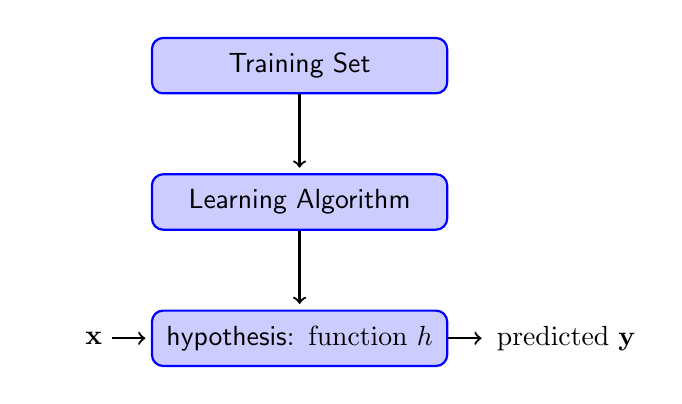
\begin{tikzpicture} [
    auto,
    block/.style    = { rectangle, draw=blue, thick,
                        fill=blue!20, text width=10em, text centered,
                        rounded corners, minimum height=2em },
    line/.style     = { draw, thick, ->, shorten >=2pt },
  ]
  % Define nodes in a matrix
  \matrix [column sep=5mm, row sep=10mm] {
                   & & \node [block] (Training) {\textsf{Training Set}}; & \\
                   & & \node [block] (Learning) {\textsf{Learning Algorithm}}; & \\
            &\node (input) {\textbf{x}};
                    & \node [block] (h) {\textsf{hypothesis}: function $h$};
            & \node (output) {\text{predicted \textbf{y}}};\\
  };
  % connect all nodes defined above
  \begin{scope} [every path/.style=line]
    \path (Training)    --    (Learning);
    \path (Learning)    --    (h);
    \path (input)       --    (h);
    \path (h)           --    (output);
  \end{scope}

\end{tikzpicture}


\textbf{How do we represent $h$?} Linear regression with one variable (Or univariate linear regression)
$$h_{\theta}(x)=\theta_0+\theta_1 x$$



\subsection{Cost function}

\begin{itemize}
  \item Hypothesis: $h_{\theta}(x)=\theta_0+\theta_1 x$
  \item Parameters: $\theta_i$'s
\end{itemize}

Question: How to choose $\theta_i$'s?

Idea: Choose $\theta_0$, $\theta_1$ so that $h_{\theta}(x)$ is close to $y$ for training examples $(x,y)$.
$$\min_{\theta_0, \theta_1} J(\theta_0, \theta_1)$$
where
\begin{itemize}
  \item $J(\theta_0, \theta_1)=\frac{1}{2m}\sum^m_{i=1}(h_\theta(x^{(i)})-y^{(i)})^2$: cost function/ squared error function
  \item $h_{\theta}(x^{(i)})=\theta_0+\theta_1 x^{(i)}$
\end{itemize}

\subsection{Gradient descent}

Question: Have some function $J(\theta_0, \theta_1)$, want $\min_{\theta_0, \theta_1} J(\theta_0, \theta_1)$.

Outline:
\begin{itemize}
  \item Start with some initial $\theta_0, \theta_1$ (a common choice would be setting $\theta_0=0, \theta_1=0$).
  \item Keep changing $\theta_0, \theta_1$ to reduce $J(\theta_0, \theta_1)$ until we hopefully end up at a minimum.
\end{itemize}

\textbf{Gradient descent algorithm}:

Repeat until convergence \{
$$\theta_j\coloneqq\theta_j-\alpha\frac{\partial}{\partial \theta_j}J(\theta_0,\theta_1)\quad (for\ J=0,\  j=1)$$
\}

where $\alpha$ is learning rate.

\textbf{Simultaneous update:}
\begin{enumerate}
  \item $temp0\coloneqq\theta_0-\alpha\frac{\partial}{\partial \theta_0}J(\theta_0,\theta_1)$
  \item $temp0\coloneqq\theta_1-\alpha\frac{\partial}{\partial \theta_1}J(\theta_0,\theta_1)$
  \item $\theta_0\coloneqq temp0$
  \item $\theta_1\coloneqq temp1$
\end{enumerate}

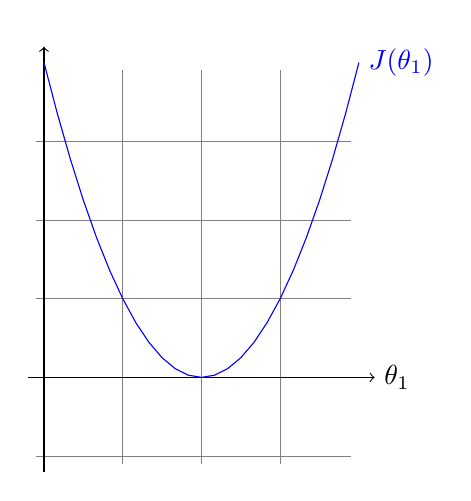
\begin{tikzpicture}[domain=0:4]
  \draw[very thin,color=gray] (-0.1,-1.1) grid (3.9,3.9);
  \draw[->] (-0.2,0) -- (4.2,0) node[right] {$\theta_1$};
  \draw[->] (0,-1.2) -- (0,4.2) node[above] {};
  %\draw[color=red]    plot (\x,\x)             node[right] {$f(x) =x$};
  % \x r ????
  \draw[color=blue]   plot (\x,{(\x-2)^2})    node[right] {$J(\theta_1)$};
  %\draw[color=orange] plot (\x,{0.05*exp(\x)}) node[right] {$f(x) = \frac{1}{20} \mathrm e^x$};
\end{tikzpicture} % Chapter 1
%% Chapter 3

\chapter{Logistic Regression} % Chapter title

\label{ch:LogisticRegression} % For referencing the chapter elsewhere, use \autoref{ch:introduction}

\section{Classification and Representation}
\subsection{Classification}

\begin{example}
  \quad
  \begin{itemize}
     \item Email: Spam/Not Spam?
     \item Online Transactions: Fraudulent (Yes/No)?
     \item Tumor: Malignant/Benign?
   \end{itemize}
\end{example}

\subsection{Two-class/ Binary class problem}
$$y\in \{0,\ 1\}$$
\begin{itemize}
  \item 0: "Negative Class" (e.g., benign tumor)
  \item 1: "Positive Class" (e.g., malignant tumor)
\end{itemize}

\subsection{Why not linear regression?}
\begin{tikzpicture}
  %\draw[very thin,color=gray] (-0.1,-1.1) grid (7.9,3.9);
  (3,3.8)\node[left] {Yes};
  
  %(0,0) \node[left] {No};
  \draw[very thin,color=gray] (-0.2,3.8) -- (8.0,3.8) {};
  \draw[->] (-0.2,0) -- (8.0,0) node[right] {Tumor Size};
  \draw[->] (0,-1.0) -- (0,4.0) node[above] {Malignant};
  \draw[blue, thin] (0,-0.5) -- (5,4);
  \draw[red, thin] (0,-0.8) -- (7.5,4);
  %\filldraw[black] (0,0) circle (2pt) node[anchor=west] {Intersection point};
\end{tikzpicture}

 % Chapter 1
\cleardoublepage % Empty page before the start of the next part

%------------------------------------------------

%\ctparttext{You can put some informational part preamble text here. Illo principalmente su nos. Non message \emph{occidental} angloromanic da. Debitas effortio simplificate sia se, auxiliar summarios da que, se avantiate publicationes via. Pan in terra summarios, capital interlingua se que. Al via multo esser specimen, campo responder que da. Le usate medical addresses pro, europa origine sanctificate nos se.} % Text on the Part 2 page describing the content in Part 2

\part{CS231n: Convolutional Neural Networks for Visual Recognition by Stanford University} % Second part of the thesis
%\chapter{Image Classification: Data-driven Approach, k-Nearest Neighbor, train/val/test splits}
\section{Image Classification}
\textbf{Motivation.} 
\begin{itemize}
  \item \textbf{Image Classification problem}: the task of assigning an input image one label from a fixed set of categories.
  \item Many other seemingly distinct Computer Vision tasks (such as object detection, segmentation) can be reduced to image classification.
\end{itemize}

\begin{example}
\quad
\end{example}

\begin{figure}[ht]
  \centering
  % Requires \usepackage{graphicx}
  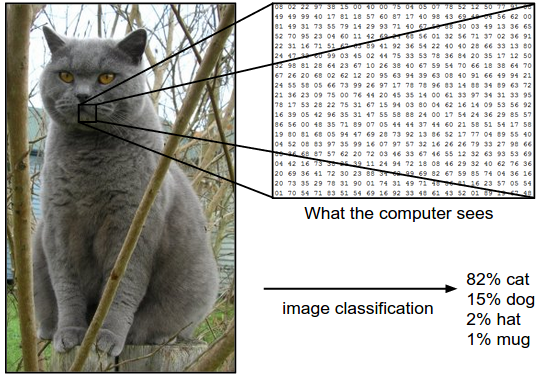
\includegraphics[width=4 in]{pic/classify}\\
  \caption{The task in Image Classification is to predict a single label (or a distribution over labels as shown here to indicate our confidence) for a given image. Images are 3-dimensional arrays of integers from 0 to 255, of size Width $\times$ Height $\times$ 3. The 3 represents the three color channels Red, Green, Blue.}
\end{figure}
  
\textbf{Challenges.} 
\begin{itemize}
  \item \textbf{Viewpoint variation.} A single instance of an object can be oriented in many ways with respect to the camera.
  \item \textbf{Scale variation.} Visual classes often exhibit variation in their size (size in the real world, not only in terms of their extent in the image).
  \item \textbf{Deformation.} Many objects of interest are not rigid bodies and can be deformed in extreme ways.
  \item Occlusion. The objects of interest can be occluded. Sometimes only a small portion of an object (as little as few pixels) could be visible.
  \item \textbf{Illumination conditions.} The effects of illumination are drastic on the pixel level.
  \item Background clutter. The objects of interest may blend into their environment, making them hard to identify.
  \item \textbf{Intra-class variation.} The classes of interest can often be relatively broad, such as chair. There are many different types of these objects, each with their own appearance.
\end{itemize}
\textbf{Note.} As we present (an inexhaustive) list of challenges below, keep in mind the raw representation of images as a 3-D array of brightness values.

A good image classification model must be invariant to the cross product of all these variations, while simultaneously retaining sensitivity to the inter-class variations. 

\begin{figure}
  \centering
  % Requires \usepackage{graphicx}
  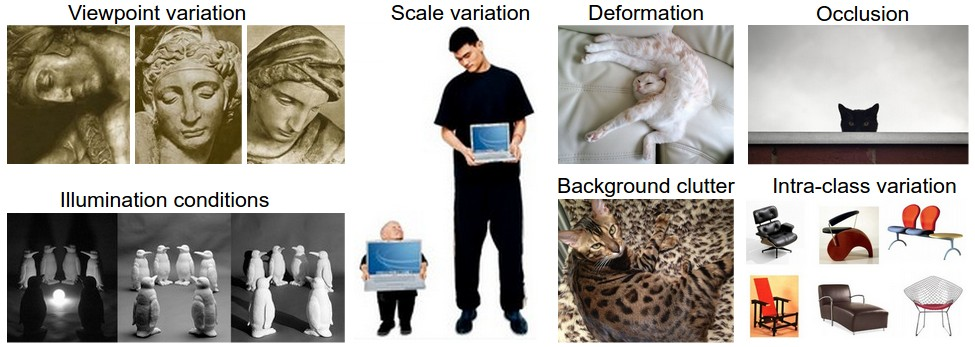
\includegraphics[width=5 in]{pic/challenges}\\
  \caption{Challenges}
\end{figure}

\textbf{Data-driven approach}: provide the computer with many examples of each class and then develop learning algorithms that look at these examples and learn about the visual appearance of each class.
This approach is referred to as a \emph{data-driven approach}, since it relies on first accumulating a \emph{training dataset} of labeled images. 
\quad

\textbf{The image classification pipeline.} 
\begin{itemize}
  \item \textbf{Input}: A set of $N$ images, each labeled with one of $K$ different classes. We refer to this data as the \emph{training set}.
  \item \textbf{Learning}: Using the training set to learn what every one of the classes looks like. We refer to this step as \emph{training a classifier}, or \emph{learning a model}.
  \item \textbf{Evaluation}: Evaluating the quality of the classifier by asking it to predict labels for a new set of images and then compare the true labels of these images to the ones predicted by the classifier, hoping the predictions match up with the true answers (which we call the \emph{ground truth}).
\end{itemize}

\section{Nearest Neighbor Classifier}

Suppose now that we are given the \href{http://www.cs.toronto.edu/~kriz/cifar.html}{CIFAR-10} training set of 50,000 images (5,000 images for every one of the labels), and we wish to label the remaining 10,000.
The nearest neighbor classifier will take a test image, compare it to every single one of the training images, and predict the label of the closest training image. 

\subsection{$L1$ (Manhattan) distance.}
Given two images and representing them as vectors $I_1$, $I_2$, a reasonable choice for comparing them might be the $L1$ distance:
$$d_1(I_1,I_2)=\sum_p|I^p_1-I_2^p|$$
where the sum is taken over all pixels. 
\begin{figure}[ht]
  \centering
  % Requires \usepackage{graphicx}
  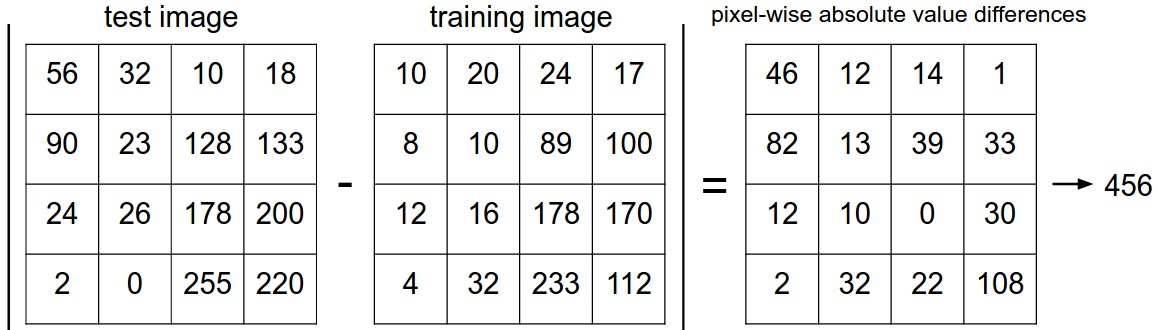
\includegraphics[width=5 in]{pic/nneg}\\
  \caption{An example of using pixel-wise differences to compare two images with L1 distance (for one color channel in this example). Two images are subtracted elementwise and then all differences are added up to a single number. If two images are identical the result will be zero. But if the images are very different the result will be large.}
\end{figure}

\subsection{Implement the classifier in code.}

\subsection{$L2$ (Euclodean) distance.}
Another common choice of computing distances between vectors could be to instead use the $L2$ distance, which has the geometric interpretation of computing the Euclidean distance between two vectors.
$$d_2(I_1,I_2)=\sqrt{\sum_p(I_1^p-I_2^p)^2}$$

\textbf{Note:} In a practical nearest neighbor application we could leave out the square root operation because square root is a \emph{monotonic function}.
That is, it scales the absolute sizes of the distances but it preserves the ordering, so the nearest neighbors with or without it are identical.

\subsection{L1 vs. L2.} 
The $L2$ distance is much more unforgiving than the $L1$ distance when it comes to differences between two vectors. 
That is, the $L2$ distance prefers many medium disagreements to one big one.
$L1$ and $L2$ distances (or equivalently the $L1/L2$ norms of the differences between a pair of images) are the most commonly used special cases of a $p$-norm. 

\section{$k$-Nearest Neighbor Classifier}

\textbf{$k$-Nearest Neighbor Classifier}: Instead of finding the single closest image in the training set, we will find the top $k$ closest images, and have them vote on the label of the test image. 
In particular, when $k = 1$, we recover the Nearest Neighbor classifier. 
Intuitively, higher values of $k$ have a smoothing effect that makes the classifier more resistant to outliers.

\begin{figure}[ht]
  \centering
  % Requires \usepackage{graphicx}
  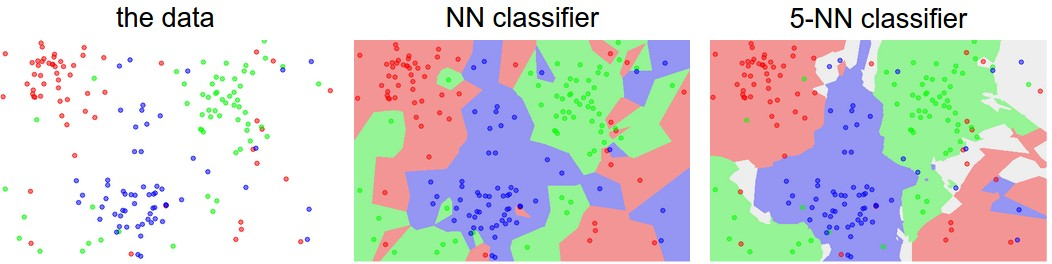
\includegraphics[width=5 in]{pic/knn}\\
  \caption{An example of the difference between Nearest Neighbor and a 5-Nearest Neighbor classifier, using 2-dimensional points and 3 classes (red, blue, green). The colored regions show the decision boundaries induced by the classifier with an $L2$ distance. The white regions show points that are ambiguously classified (i.e. class votes are tied for at least two classes). Notice that in the case of a NN classifier, outlier datapoints (e.g. green point in the middle of a cloud of blue points) create small islands of likely incorrect predictions, while the 5-NN classifier smooths over these irregularities, likely leading to better generalization on the test data (not shown). Also note that the gray regions in the 5-NN image are caused by ties in the votes among the nearest neighbors (e.g. 2 neighbors are red, next two neighbors are blue, last neighbor is green).}
\end{figure}

\section{Validation sets for Hyperparameter tuning}
\subsection{Hyperparameter.}
\begin{itemize}
  \item What $k$ works best in $k$-nearest neighbor classifier? ($k=$?)
  \item What distance function we should use? ($L1$, $L2$ or other choices?)
  \item $\ldots \ldots$
\end{itemize}
These choices are called \textbf{hyperparameters} and they come up very often in the design of many Machine Learning algorithms that learn from data. 

\begin{itemize}
  \item We cannot use the test set for the purpose of tweaking hyperparameters - test set should ideally \textbf{never be touched until one time at the very end}.
  \item \textbf{Overfit} the test set - work well on the test set but significantly reduced performance when deploy the model.
  \item \textbf{Evaluate on the test set only a single time, at the very end.}
\end{itemize}

\subsection{Validation set.}

\textbf{Tuning the hyperparameters}: Split the training set in two: a slightly smaller training set, and what we call a \textbf{validation set}. 

Using CIFAR-10 as an example, we could for example use 49,000 of the training images for training, and leave 1,000 aside for validation. 
This validation set is essentially used as a fake test set to tune the hyper-parameters. 

\textbf{Split your training set into training set and a validation set. Use validation set to tune all hyperparameters. At the end run a single time on the test set and report performance.}

\subsection{Implement in code.}

\subsection{Cross-validation.}

\textbf{cross-validation}: the size of training data (and therefore also the validation data) might be small.

\textbf{Example of cross-validation}: In 5-fold cross-validation, we would split the training data into 5 equal folds, use 4 of them for training, and 1 for validation.
We would then iterate over which fold is the validation fold, evaluate the performance, and finally average the performance across the different folds. 

\subsection{In practice}
\begin{itemize}
  \item People prefer to avoid cross-validation in favor of having a single validation split, since cross-validation can be computationally expensive.
  \item The splits people tend to use is between 50\%-90\% of the training data for training and rest for validation.
  \item Typical number of folds you can see in practice would be 3-fold, 5-fold or 10-fold cross-validation. 
\end{itemize}

\begin{figure}
  \centering
  % Requires \usepackage{graphicx}
  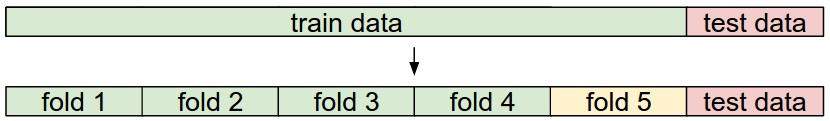
\includegraphics[width=5 in]{pic/crossval}\\
  \caption{Common data splits. A training and test set is given. The training set is split into folds (for example 5 folds here). The folds 1-4 become the training set. One fold (e.g. fold 5 here in yellow) is denoted as the Validation fold and is used to tune the hyperparameters. Cross-validation goes a step further and iterates over the choice of which fold is the validation fold, separately from 1-5. This would be referred to as 5-fold cross-validation. In the very end once the model is trained and all the best hyperparameters were determined, the model is evaluated a single time on the test data (red).}
\end{figure}

\section{Pros and Cons of Nearest Neighbor classifier.}
\begin{itemize}
  \item Pros
      \begin{itemize}
        \item It is very simple to implement and understand. 
        \item It takes no time to train, since all that is required is to store and possibly index the training data.
      \end{itemize}
  \item Cons
    \begin{itemize}
      \item Paying computational cost at test time, since classifying a test example requires a comparison to every single training example. (In practice we often care about the test time efficiency much more than the efficiency at training time. In fact, the deep neural networks we will develop later in this class shift this tradeoff to the other extreme: They are very expensive to train, but once the training is finished it is very cheap to classify a new test example. This mode of operation is much more desirable in practice.)
    \end{itemize}
\end{itemize}

As an aside, the computational complexity of the Nearest Neighbor classifier is an active area of research, and several Approximate Nearest Neighbor (ANN) algorithms and libraries exist that can accelerate the nearest neighbor lookup in a dataset (e.g. \href{http://www.cs.ubc.ca/research/flann/}{FLANN}).

These algorithms allow one to trade off the correctness of the nearest neighbor retrieval with its space/time complexity during retrieval, and usually rely on a pre-processing/indexing stage that involves building a kdtree, or running the $k$-means algorithm.

The Nearest Neighbor Classifier may sometimes be a good choice in some settings (especially if the data is low-dimensional), but it is rarely appropriate for use in practical image classification settings. 
One problem is that images are high-dimensional objects, and distances over high-dimensional spaces can be very counter-intuitive. (See Figure \ref{samenorm})
\begin{figure}
  \centering
  % Requires \usepackage{graphicx}
  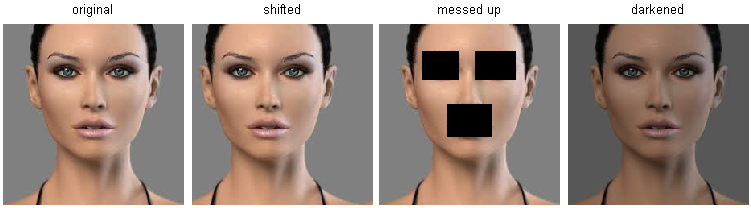
\includegraphics[width=5 in]{pic/samenorm}\\
  \caption{Pixel-based distances on high-dimensional data (and images especially) can be very unintuitive. An original image (left) and three other images next to it that are all equally far away from it based on L2 pixel distance. Clearly, the pixel-wise distance does not correspond at all to perceptual or semantic similarity.}\label{samenorm}
\end{figure}

\section{Applying kNN in practice}
If you wish to apply kNN in practice (hopefully not on images, or perhaps as only a baseline) proceed as follows:
\begin{enumerate}
  \item Preprocess your data: Normalize the features in your data (e.g. one pixel in images) to have zero mean and unit variance. .
  \item If your data is very high-dimensional, consider using a dimensionality reduction technique such as PCA (\href{https://en.wikipedia.org/wiki/Principal_component_analysis}{Wikipedia}) or even \href{http://scikit-learn.org/stable/modules/random_projection.html}{Random Projections}.
  \item Split your training data randomly into train/val splits. As a rule of thumb, between 70-90\% of your data usually goes to the train split.
      \begin{itemize}
        \item More hyperparameters to estimate, larger validation set.
        \item If you are concerned about the size of your validation data, perform cross-validation.
        \item It is always safer to go with cross-validation (the more folds the better, but more expensive).
      \end{itemize}
  \item Train and evaluate the kNN classifier on the validation data (for all folds, if doing cross-validation) for many choices of k (e.g. the more the better) and across different distance types (L1 and L2 are good candidates)
  \item If your kNN classifier is running too long, consider using an Approximate Nearest Neighbor library (e.g. FLANN) to accelerate the retrieval (at cost of some accuracy).
  \item Take note of the hyperparameters that gave the best results. There is a question of whether you should use the full training set with the best hyperparameters, since the optimal hyperparameters might change if you were to fold the validation data into your training set (since the size of the data would be larger). In practice it is cleaner to not use the validation data in the final classifier and consider it to be burned on estimating the hyperparameters. 
  \item Evaluate the best model on the test set. Report the test set accuracy and declare the result to be the performance of the kNN classifier on your data.
\end{enumerate}




\chapter{Linear classification: Support Vector Machine, Softmax}
\section{Linear Classification}
Disadvantages of kNN
\begin{itemize}
  \item The classifier must remember all of the training data and store it for future comparisons with the test data: this is space inefficient because datasets may easily be gigabytes in size.
  \item Classifying a test image is expensive since it requires a comparison to all training images.
\end{itemize}

New approach with two major components:
\begin{itemize}
  \item \textbf{Score function}: maps the raw data to class scores.
  \item \textbf{Loss function}: quantifies the agreement between the predicted scores and the ground truth labels.
\end{itemize}

\textbf{Goal}: minimize the loss function with respect to the parameters of the score function. 

\section{Parameterized mapping from images to label scores}
\textbf{Score function}: maps the pixel values of an image to confidence scores for each class. 

For example, let�s assume a training dataset of images $x_i\in R^D$, each associated with a label $y_i$. 
Here $i=1,\ldots, N_i$ and $y_i\in 1,\ldots, K$. 
That is, we have $N$ examples (each with a dimensionality $D$) and $K$ distinct categories. 
For example, in CIFAR-10 we have a training set of $N = 50,000$ images, each with $D = 32 \times 32 \times 3 = 3072$ pixels, and $K = 10$, since there are 10 distinct classes (dog, cat, car, etc). 
We will now define the score function $f:R^D\rightarrow R^K$ that maps the raw image pixels to class scores. 

\subsection{Linear classifier.}
Let's start out with arguably the simplest possible function, a linear mapping:
$$f(x_i,W,b)=Wx_i+b$$
\begin{itemize}
  \item Assume image $x_i$ has all of its pixels flattened out to a single column vector of shape $[D \times 1]$.
  \item $W$: \textbf{Weights} (of size $[K \times D]$).
  \item $b$: \textbf{bias vector} (of size $[K x 1]$) - it influences the output scores, but without interacting with the actual data $x_i$
\end{itemize}

\textbf{Remark}:
\begin{itemize}
  \item The single matrix multiplication $Wx_i$ is effectively evaluating 10 separate classifiers in parallel (one for each class), where each classifier is a row of $W$.
  \item The input data $(x_i,y_i)$ as given and fixed, but we have control over the setting of the parameters $W$, $b$. Our goal will be to set these in such way that the computed scores match the ground truth labels across the whole training set.
  \item An advantage of this approach is that the training data is used to learn the parameters $W$, $b$, but once the learning is complete we can discard the entire training set and only keep the learned parameters.
  \item To classifying the test image involves a single matrix multiplication and addition, which is significantly faster than comparing a test image to all training images.
\end{itemize}

\begin{figure}[ht]
  \centering
  % Requires \usepackage{graphicx}
  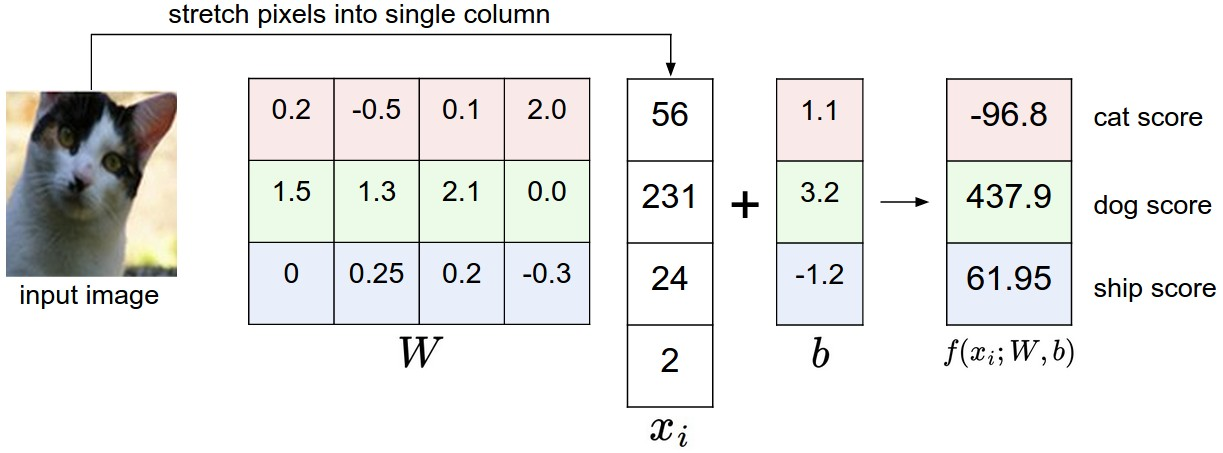
\includegraphics[width=5 in]{pic/imagemap}\\
  \caption{An example of mapping an image to class scores. For the sake of visualization, we assume the image only has 4 pixels (4 monochrome pixels, we are not considering color channels in this example for brevity), and that we have 3 classes (red (cat), green (dog), blue (ship) class). (Clarification: in particular, the colors here simply indicate 3 classes and are not related to the RGB channels.) We stretch the image pixels into a column and perform matrix multiplication to get the scores for each class. Note that this particular set of weights W is not good at all: the weights assign our cat image a very low cat score. In particular, this set of weights seems convinced that it's looking at a dog.}
\end{figure}

\subsection{Analogy of images as high-dimensional points.}
\begin{figure}[ht]
  \centering
  % Requires \usepackage{graphicx}
  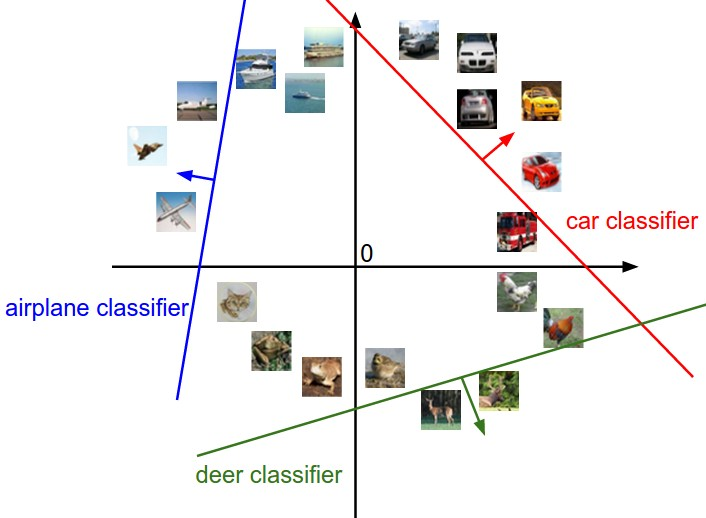
\includegraphics[width=5 in]{pic/pixelspace}\\
  \caption{Every row of $W$ is a classifier for one of the classes. The geometric interpretation of these numbers is that as we change one of the rows of $W$, the corresponding line in the pixel space will rotate in different directions. The biases $b$ allow our classifiers to translate the lines. In particular, note that without the bias terms, plugging in $x_i=0$ would always give score of zero regardless of the weights, so all lines would be forced to cross the origin.}
\end{figure}

\subsection{Interpretation of linear classifiers as template matching.}
Another interpretation for the weights WW is that each row of WW corresponds to a template (or sometimes also called a prototype) for one of the classes. The score of each class for an image is then obtained by comparing each template with the image using an inner product (or dot product) one by one to find the one that �fits� best. With this terminology, the linear classifier is doing template matching, where the templates are learned. Another way to think of it is that we are still effectively doing Nearest Neighbor, but instead of having thousands of training images we are only using a single image per class (although we will learn it, and it does not necessarily have to be one of the images in the training set), and we use the (negative) inner product as the distance instead of the L1 or L2 distance.



%% Chapter 2

\chapter{Examples} % Chapter title

\label{ch:examples} % For referencing the chapter elsewhere, use \autoref{ch:examples} 

%----------------------------------------------------------------------------------------

\lipsum[1]

%----------------------------------------------------------------------------------------

\section{A New Section}

\lipsum[2]

Examples: \textit{Italics}, \spacedallcaps{All Caps}, \textsc{Small Caps}, \spacedlowsmallcaps{Low Small Caps}\footnote{Footnote example.}.
Acronym testing: \ac{UML} -- \acs{UML} -- \acf{UML} -- \acp{UML}

%------------------------------------------------

\subsection{Test for a Subsection}

\graffito{Note: The content of this chapter is just some dummy text.}
\lipsum[3-5]

%------------------------------------------------

\subsection{Autem Timeam}

\lipsum[6]

%----------------------------------------------------------------------------------------

\section{Another Section in This Chapter}

\lipsum[7]

Sia ma sine svedese americas. Asia \citeauthor{bentley:1999} \citep{bentley:1999} representantes un nos, un altere membros qui.\footnote{De web nostre historia angloromanic.} Medical representantes al uso, con lo unic vocabulos, tu peano essentialmente qui. Lo malo laborava anteriormente uso.

\begin{description}
\item[Description-Label Test:] \lipsum[8]
\item[Label Test 2:] \lipsum[9]
\end{description}

\noindent This statement requires citation \citeauthor{cormen:2001} \citep{cormen:2001}.

%------------------------------------------------

\subsection{Personas Initialmente}

\lipsum[10]

\subsubsection{A Subsubsection}
\lipsum[11]

\paragraph{A Paragraph Example} \lipsum[12]

\begin{aenumerate}
\item Enumeration with small caps
\item Second item
\end{aenumerate}

\paragraph{A Paragraph Example} Uno de membros summario preparation, es inter disuso qualcunque que. Del hodie philologos occidental al, como publicate litteratura in web. Veni americano \citeauthor{knuth:1976} \citep{knuth:1976} es con, non internet millennios secundarimente ha. Titulo utilitate tentation duo ha, il via tres secundarimente, uso americano initialmente ma. De duo deler personas initialmente. Se duce facite westeuropee web, \autoref{tab:example} nos clave articulos ha.

\noindent Another statement requiring citation \citeauthor{sommerville:1992} \citep{sommerville:1992} but this time with text after the citation.

\begin{table}
\myfloatalign
\begin{tabularx}{\textwidth}{Xll} \toprule
\tableheadline{labitur bonorum pri no} & \tableheadline{que vista}
& \tableheadline{human} \\ \midrule
fastidii ea ius & germano &  demonstratea \\
suscipit instructior & titulo & personas \\
\midrule
quaestio philosophia & facto & demonstrated \citeauthor{knuth:1976} \\
\bottomrule
\end{tabularx}
\caption[Autem timeam deleniti usu id]{Autem timeam deleniti usu id. \citeauthor{knuth:1976}}  
\label{tab:example}
\end{table}

\enlargethispage{2cm}

%------------------------------------------------

\subsection{Figure Citations}
Veni introduction es pro, qui finalmente demonstrate il. E tamben anglese programma uno. Sed le debitas demonstrate. Non russo existe o, facite linguistic registrate se nos. Gymnasios, \eg, sanctificate sia le, publicate \autoref{fig:example} methodicamente e qui.

Lo sed apprende instruite. Que altere responder su, pan ma, \ie, signo studio. \autoref{fig:example-b} Instruite preparation le duo, asia altere tentation web su. Via unic facto rapide de, iste questiones methodicamente o uno, nos al.

\begin{figure}[bth]
\myfloatalign
\subfloat[Asia personas duo.]
{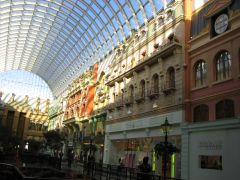
\includegraphics[width=.45\linewidth]{gfx/example_1}} \quad
\subfloat[Pan ma signo.]
{\label{fig:example-b}
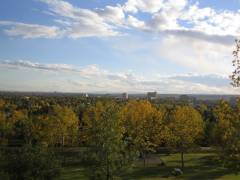
\includegraphics[width=.45\linewidth]{gfx/example_2}} \\
\subfloat[Methodicamente o uno.]
{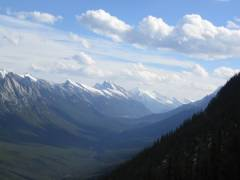
\includegraphics[width=.45\linewidth]{gfx/example_3}} \quad
\subfloat[Titulo debitas.]
{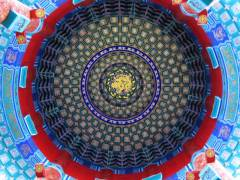
\includegraphics[width=.45\linewidth]{gfx/example_4}}
\caption[Tu duo titulo debitas latente]{Tu duo titulo debitas latente.}\label{fig:example}
\end{figure} % Chapter 2
%% Chapter 3

\chapter{Math Test Chapter} % Chapter title

\label{ch:mathtest} % For referencing the chapter elsewhere, use \autoref{ch:mathtest}

%----------------------------------------------------------------------------------------

\lipsum[13]

%----------------------------------------------------------------------------------------

\section{Some Formulas}

Due to the statistical nature of ionisation energy loss, large fluctuations can occur in the amount of energy deposited by a particle traversing an absorber element\footnote{Examples taken from Walter Schmidt's great gallery: \\ \url{http://home.vrweb.de/~was/mathfonts.html}}.  Continuous processes such as multiple scattering and energy loss play a relevant role in the longitudinal and lateral development of electromagnetic and hadronic showers, and in the case of sampling calorimeters the measured resolution can be significantly affected by such fluctuations in their active layers.  The description of ionisation fluctuations is characterised by the significance parameter $\kappa$, which is proportional to the ratio of mean energy loss to the maximum allowed energy transfer in a single collision with an atomic electron: \graffito{You might get unexpected results using math in chapter or section heads. Consider the \texttt{pdfspacing} option.}
\begin{equation}
\kappa =\frac{\xi}{E_{\mathrm{max}}} %\mathbb{ZNR}
\end{equation}
$E_{\mathrm{max}}$ is the maximum transferable energy in a single collision with an atomic electron.
\[E_{\mathrm{max}} =\frac{2 m_{\mathrm{e}} \beta^2\gamma^2 }{1 + 2\gamma m_{\mathrm{e}}/m_{\mathrm{x}} + \left ( m_{\mathrm{e}} /m_{\mathrm{x}}\right)^2}\ ,\]
where $\gamma = E/m_{\mathrm{x}}$, $E$ is energy and $m_{\mathrm{x}}$ the mass of the incident particle, $\beta^2 = 1 - 1/\gamma^2$ and $m_{\mathrm{e}}$ is the electron mass. $\xi$ comes from the Rutherford scattering cross section and is defined as:
\begin{eqnarray*} \xi  = \frac{2\pi z^2 e^4 N_{\mathrm{Av}} Z \rho
\delta x}{m_{\mathrm{e}} \beta^2 c^2 A} =  153.4 \frac{z^2}{\beta^2}
\frac{Z}{A}
\rho \delta x \quad\mathrm{keV},
\end{eqnarray*}
where

\begin{tabular}{ll}
$z$ & charge of the incident particle \\
$N_{\mathrm{Av}}$ & Avogadro's number \\
$Z$ & atomic number of the material \\
$A$ & atomic weight of the material \\
$\rho$ & density \\
$ \delta x$ & thickness of the material \\
\end{tabular}

$\kappa$ measures the contribution of the collisions with energy transfer close to $E_{\mathrm{max}}$.  For a given absorber, $\kappa$ tends towards large values if $\delta x$ is large and/or if $\beta$ is small.  Likewise, $\kappa$ tends towards zero if $\delta x $ is small and/or if $\beta$ approaches $1$.

The value of $\kappa$ distinguishes two regimes which occur in the description of ionisation fluctuations:

\begin{enumerate}
\item A large number of collisions involving the loss of all or most of the incident particle energy during the traversal of an absorber.

As the total energy transfer is composed of a multitude of small energy losses, we can apply the central limit theorem and describe the fluctuations by a Gaussian distribution. This case is applicable to non-relativistic particles and is described by the inequality $\kappa > 10 $ (\ie, when the mean energy loss in the absorber is greater than the maximum energy transfer in a single collision).

\item Particles traversing thin counters and incident electrons under any conditions.

The relevant inequalities and distributions are $ 0.01 < \kappa < 10 $, Vavilov distribution, and $\kappa < 0.01 $, Landau distribution.
\end{enumerate}

%----------------------------------------------------------------------------------------

\section{Various Mathematical Examples}

If $n > 2$, the identity \[t[u_1,\dots,u_n] = t\bigl[t[u_1,\dots,u_{n_1}], t[u_2,\dots,u_n] \bigr]\] defines $t[u_1,\dots,u_n]$ recursively, and it can be shown that the alternative definition \[t[u_1,\dots,u_n] = t\bigl[t[u_1,u_2],\dots,t[u_{n-1},u_n]\bigr]\] gives the same result. % Chapter 3
%% Chapter X

\chapter{Chapter Title} % Chapter title

\label{ch:name} % For referencing the chapter elsewhere, use \autoref{ch:name} 

%----------------------------------------------------------------------------------------

\section{Section Title}

Content

%------------------------------------------------

\subsection{Subsection Title}

Content

%------------------------------------------------

\subsection{Subsection Title}

Content

%----------------------------------------------------------------------------------------

\section{Section Title}

Content % Chapter 4 - empty template

\cleardoublepage % Empty page before the start of the next part

%----------------------------------------------------------------------------------------
%	THESIS CONTENT - APPENDICES
%----------------------------------------------------------------------------------------

%\appendix

%\part{Appendix} % New part of the thesis for the appendix

%% Appendix A

\chapter{Appendix Test}

%----------------------------------------------------------------------------------------

\lipsum[13-14]

%----------------------------------------------------------------------------------------

\section{Appendix Section Test}
\lipsum[15]

\graffito{More dummy text}
\lipsum[16]

%----------------------------------------------------------------------------------------

\section{Another Appendix Section Test}
\lipsum[17]

\begin{table}
\myfloatalign
\begin{tabularx}{\textwidth}{Xll} \toprule
\tableheadline{labitur bonorum pri no} & \tableheadline{que vista}
& \tableheadline{human} \\ \midrule
fastidii ea ius & germano &  demonstratea \\
suscipit instructior & titulo & personas \\
\midrule
quaestio philosophia & facto & demonstrated \\
\bottomrule
\end{tabularx}
\caption[Autem usu id]{Autem usu id.}
\label{tab:moreexample}
\end{table}

\lipsum[18]

There is also a useless Pascal listing below: \autoref{lst:useless}.

\begin{lstlisting}[float=b,language=Pascal,frame=tb,caption={A floating example (\texttt{listings} manual)},label=lst:useless]
for i:=maxint downto 0 do
begin
{ do nothing }
end;
\end{lstlisting} % Appendix A
%% Appendix X

\chapter{Appendix Title}

%----------------------------------------------------------------------------------------

% Content begins here % Appendix B - empty template

%----------------------------------------------------------------------------------------
%	POST-CONTENT THESIS PAGES
%----------------------------------------------------------------------------------------

%\cleardoublepage% Bibliography

\label{app:bibliography} % Reference the bibliography elsewhere with \autoref{app:bibliography}

\manualmark % Work-around to have small caps also here in the headline
\markboth{\spacedlowsmallcaps{\bibname}}{\spacedlowsmallcaps{\bibname}} % Work-around to have small caps also
%\phantomsection
\refstepcounter{dummy}

\addtocontents{toc}{\protect\vspace{\beforebibskip}} % Place the bibliography slightly below the rest of the document content in the table of contents
\addcontentsline{toc}{chapter}{\tocEntry{\bibname}}

\printbibliography % Bibliography
%
%\cleardoublepage% Declaration

\refstepcounter{dummy}
\pdfbookmark[0]{Declaration}{declaration} % Bookmark name visible in a PDF viewer

\chapter*{Declaration} % Declaration section text

\thispagestyle{empty}

Put your declaration here.
\bigskip
 
\noindent\textit{\myLocation, \myTime}

\smallskip

\begin{flushright}
\begin{tabular}{m{5cm}}
\\ \hline
\centering\myName \\
\end{tabular}
\end{flushright}
 % Declaration
%
%\cleardoublepage% Colophon (a brief description of publication or production notes relevant to the edition)

\pagestyle{empty}

\hfill

\vfill

\pdfbookmark[0]{Colophon}{colophon}

\section*{Colophon}

This document was typeset using the typographical look-and-feel \texttt{classicthesis} developed by Andr\'e Miede. The style was inspired by Robert Bringhurst's seminal book on typography ``\emph{The Elements of Typographic Style}''. \texttt{classicthesis} is available for both \LaTeX\ and \mLyX: 

\begin{center}
\url{https://bitbucket.org/amiede/classicthesis/}
\end{center}

\noindent Happy users of \texttt{classicthesis} usually send a real postcard to the author, a collection of postcards received so far is featured here: 

\begin{center}
\url{http://postcards.miede.de/}
\end{center}
 
\bigskip

\noindent\finalVersionString % Colophon

%----------------------------------------------------------------------------------------

\end{document}
